\uuid{9AEq}
\exo7id{7598}
\auteur{mourougane}
\organisation{exo7}
\datecreate{2021-08-10}
\isIndication{false}
\isCorrection{true}
\chapitre{Autre}
\sousChapitre{Autre}

\contenu{
\texte{

}
\begin{enumerate}
    \item \question{Peut on définir une détermination de la fonction logarithme sur $ \mathbb{C} \backslash \{ \; x \in \Rr \; / \; x \geq 0 \;\} $ ? 
Dans le cas affirmatif, donner une définition de cette détermination. 


%}
    \item \question{Plus généralement peut on définir une détermination du logarithme sur le plan complexe privé d'une demi droite quelconque issue de l'origine ?}
    \item \question{M\^ eme question sur le plan complexe privé de l'ensemble $$ L=[ \; 0,1\; ] \cup \{ \; z \in \mathbb{C} \; / \; \mid z-2 \mid =1  \; {et} \; Im(z) \geq 0 \; \} \cup [\; 3, \infty \; [ .$$


$$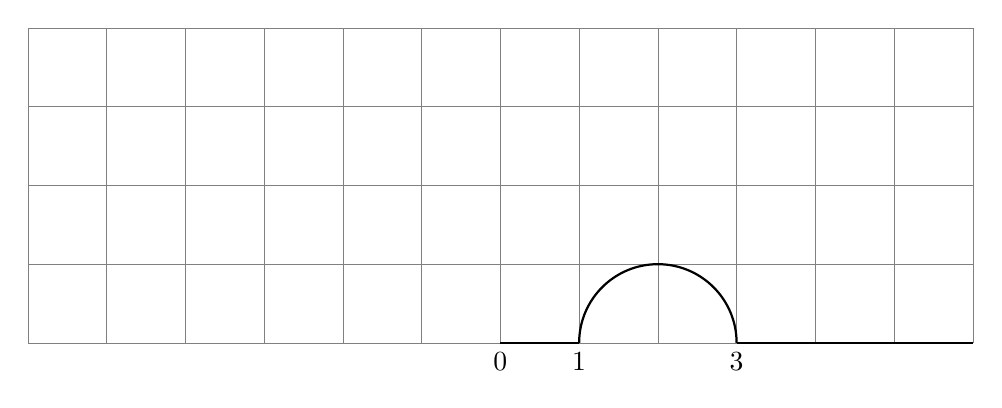
\begin{tikzpicture}
\draw[help lines, step=1, very thin] (-6,0) grid (6,4);
\draw[shift={(3,0)}, thick] (2:0) arc (0:180:1cm);
\draw[thick] (0,0) -- (1,0) ;\draw[thick] (3,0) -- (6,0) ;
\draw (0,0) node[below]{$0$} ;
\draw (3,0) node[below]{$3$} ;
\draw (1,0) node[below]{$1$} ;
\end{tikzpicture}$$}
\reponse{
On définit une détermination du logarithme en posant
$$\begin{array}{cccc}
 l_+ :& \Cc-[0,+\infty[ & \longrightarrow & \Cc\\ & z=re^{i\theta} (r>0, 0<\theta<2\pi)&\longmapsto& \log_\Rr(r)+i\theta.
\end{array}$$
On définit une détermination du logarithme en posant
$$\begin{array}{cccc}
 \ell :& \Cc-L & \longrightarrow & \Cc\\ & z=re^{i\theta} (r>0, 0\leq\theta<2\pi)&\longmapsto& 
 \left\{\begin{array}{l} \textrm{si }\mid z-2 \mid \leq 1 \quad \text{ et } \quad  Im(z) \geq 0, \\ \ \ \ \ \ell(z)=\log_\Rr(r)+i(\theta +2\pi).\\
 \textrm{si }\mid z-2 \mid > 1, \\ \ \ \ \ \ell(z)=\log_\Rr(r)+i\theta\end{array}
 \right.
\end{array}$$
On vérifie que $\ell$ est continue : en particulier sur le disque ouvert de centre $(2,0)$ et de rayon $1$, $\ell$ coïncide avec la fonction $\log +2i\pi$,
qui est continue. 
On vérifie aussi que pour tout $z\in\Cc-L$, $e^{\ell(z)}=z$ : c'est donc une détermination du logarithme sur $\Cc-L$.
}
\end{enumerate}
}
